\documentclass[12pt]{article}
\usepackage{lineno, blindtext,  enumerate, algorithmic }
\usepackage{amssymb}
\usepackage{hyperref}
\usepackage{amsthm}
\usepackage{amsmath}
\usepackage{natbib}
\usepackage{graphicx}
% \usepackage[sorting=none]{biblatex}
\usepackage{enumitem}
\renewcommand{\baselinestretch}{1.0}
% \setlength{\oddsidemargin}{0.0in}
% \setlength{\evensidemargin}{0.0in}
% \setlength{\topmargin}{0.0in}
% \setlength{\textheight}{8.5in}
% \setlength{\textwidth}{6.5in}
\usepackage[letterpaper]{geometry}
\geometry{top=1.0in, bottom=1.0in, left=1.0in, right=1.0in}
\setlength{\headsep}{0in}
\setlength{\parindent}{0in}
\usepackage{setspace}
\doublespacing
\newcommand{\utwi}[1]{\mbox{\boldmath $ #1$}}
\pagestyle{plain}
\includeonly{}

\newcommand\blfootnote[1]{%
  \begingroup
  \renewcommand\thefootnote{}\footnote{#1}%
  \addtocounter{footnote}{-1}%
  \endgroup
}

% \bibliography{references}

\begin{document}

\begin{center}
{\bf RICE UNIVERSITY} \\
STAT 525 \\
{\it Bayesian Statistics} \\ 
\vspace{5pt}
Shashank Sonkar \\
\vspace{11pt}
{\bf Project Report}
\end{center}

\section{Introduction}
Let us say we are given some questions, and students' responses to these questions (responses are either marked correct or incorrect). Given this information, one of the most important tasks in the field of educational data mining is to predict each question's (also called an item) difficulty and each student's proficiency. Rasch laid the foundation of item response theory (IRT) in around 1960s \cite{rasch1960probabilistic,rasch1966item}. Using Markov Chain Monte Carlo (MCMC) methods, one can estimate the item difficulty and student proficiency parameters.

However, one of the main drawbacks of the IRT models is the lack of interpretability. To alleviate this drawback, the paper under review for this project \cite{fox2001bayesian} provides an elegant multilevel extension to traditional IRT models. This paper extends the standard IRT model further by grouping students into schools, and proposing a multilevel regression model to study the properties of groups (e.g. schools, in this case) as well. It adopts a fully Bayesian approach, unlike its predecessors, that provides it benefits like uncertainty quantification, and ease of incorporating information about schools through priors.

% \section{Main topics to be covered:}
% \begin{enumerate}[label=(\alph*)]
%     \item Understand standard IRT models
%     \item Understand the assumption of homoscedasticity in standard IRT models that the paper tries to alleviate.
%     \item Understand two-Level one-way random effects ANOVA model.
%     \item Study how the above model can be used to model the multilevel extension to the standard IRT model.
%     \item Understand the estimation of multilevel IRT model parameters using Gibbs sampling.
%     \item Implement the model in Stan.
%     \item Run the R and Stan models on PISA 2003 dataset to compare the two implementations, and also test the model's performance on a bigger dataset (since, authors analyzed an older, smaller PISA dataset in the paper).
% \end{enumerate}

% \section{Points to mention}
% \begin{itemize}
%     \item IRT models do not explain - multilevel IRT models are an attempt to integrate at least some interpretability.
    
%     pg 5- (See Appendix E, “Linear Logistic Test Model [LLTM],” for a brief presentation of one of these explanatory approaches, as well as De Boeck \& Wilson [2004] for alternative approaches.) The cognitive processes used by an individual to respond to an item are not modeled in the commonly used IRT models. In short, this approach is analogous to measuring the speed of an automobile without understanding how an automobile moves. \cite{de2013theory}
    
%     \item  Use these values as priors.
    
%     pg 15 - However, typical item and person locations fall within –3 to 3 \cite{de2013theory}.
    
%     pg 101 - Reasonably good values of $\alpha$ range from approximately 0.8 to about 2.5 \cite{de2013theory}.
% \end{itemize}

\section{Project Outline and Contributions}
We start by understanding the conceptual development of IRT models in section \ref{sec:xpl_irt}. One key idea, that we understood by taking this route, is the decision to either use the normal ogive or the logit function to model the success probability of a student's response to an item. Rasch model, 1-PL, 2-PL, and 3-PL models use the logit function, while the paper under review for this project \cite{fox2001bayesian} uses the normal ogive function.

We list down the full conditionals for the normal ogive model, derived in \cite{fox2001bayesian}, in section \ref{sec:full_conditionals_mlirt}. To explore the multilevel IRT models through the lens of the logit function, and not just normal ogive function \cite{fox2001bayesian}, we use Stan which provides us with the flexibility to model a logit multilevel IRT model without deriving the full conditionals.

We experiment on a small dataset \cite{thissen1993detection} for which the Stan implementation of 2PL logit multilevel model is open-source \cite{furr2016two}. We can easily modify the codebase for normal ogive model to replicate \cite{fox2001bayesian}, and compare the two models. The primary motivation to compare the two models is to check which one of the two - logit or normal-ogive, provides a better fit to the data.

For implementations in Stan, \cite{furr2016two} highlights the importance of non-centered parametrization for hierarchical models (see \cite{papaspiliopoulos2007general} for in-depth review). In our experiments, we also test the impact of non-centered parametrization on effective sample size in the case of normal ogive 2PL multilevel model.

Our experiments to run the models on the larger PISA 2003 dataset were unsuccessful, mainly because of the huge running time needed for successful convergence. Efforts to install and run the package (/source code) of `mlirt' in R provided by the author of \cite{fox2001bayesian} in 2007 \cite{fox2007multilevel} did not pay off. However, we could extract the code required to pre-process and load the 2003 PISA dataset from the `mlirt' package source code.

% Stan models to compare the multilevel normal ogive and logit models on PISA 2003 dataset are provided (tested for few chains and iterations), but the analysis is incomplete due to the running time needed for successful convergence.

\section{Conceptual Development of x-PL IRT Models} \label{sec:xpl_irt}

This section is based on the readings of chapter 1, 2, 5, and 6 of \cite{de2013theory}.

\subsection{1-PL IRT Model}
In an IRT model, one estimates the properties of the item which are responsible for the differing responses to that item. In education, these items are generally questions. In the 1-PL model, the most characteristic of the item is measured, which is the difficulty of the item. The probability that a student will answer $j^{th}$ item correctly is modeled by:

\begin{equation}\label{eq:1pl}
    P(y_j=1|\theta, \delta_j) = \frac{e^{\theta - \delta_j}}{1+e^{\theta - \delta_j}},
\end{equation}
where $y_j$ models the correctness of the response of the student to item $j$ (1 if correct, 0 otherwise),  $\theta$ is the student's ability parameter, and $\delta_j$ is the item' difficulty parameter.

\subsection{2-PL IRT Model}
One can observe from \eqref{eq:1pl} that when a student's ability parameter, $\theta$, is equal to $\delta_j$, the probability of the student answering the question $j$ correctly is $0.5$. As $\theta$ moves away from $\delta_j$, the change in success probability ($dP/ d\theta) $ is not a function of the item (sigmoid function only gets shifted by $\delta_j$). However, in educational settings, some items may require a large change in $\theta$ to achieve some fixed change in success probability from $0.5$. To elucidate, $\delta_j$ is fixed at 1 in figure \ref{fig:2pl}. The blue line indicates the change in success probability across item 1 and item 2, when the ability parameter of the student changes from 1 to 2. Thus, item 1 is said to be better at `discriminating' students (more sensitive to $\theta$), since a large change in $\theta$ is needed for the same increase in success probability from 0.5.

\begin{figure}[t]
    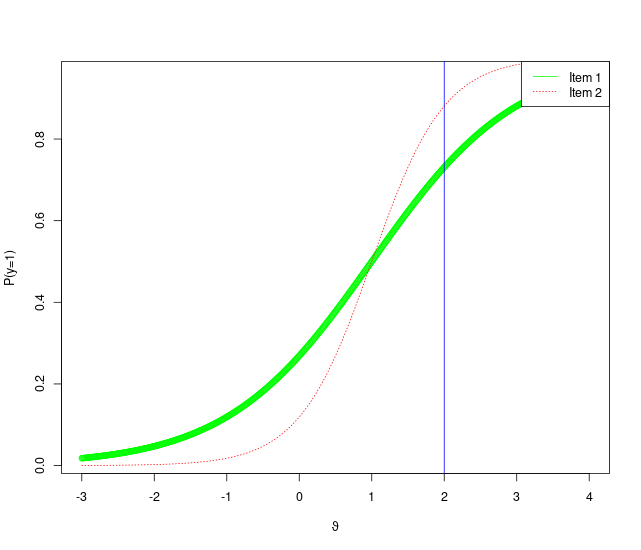
\includegraphics[scale=0.5]{Plots/2pl.png}
    \centering
    \caption{2PL model}
    \label{fig:2pl}
\end{figure}

The probability that a student will answer $j^{th}$ item correctly in the 2PL model is modeled by:

\begin{equation}\label{eq:2pl}
    P(y_j=1|\theta, \delta_j, \alpha_j) = \frac{e^{\alpha_j(\theta - \delta_j)}}{1+e^{\alpha_j(\theta - \delta_j)}},
\end{equation}
where $\alpha_j$ is the item's discrimination parameter.

\textbf{Note on use of sigmoid and its ramifications for multilevel IRT models:}

Fitting the probability of the correct response using the sigmoid function is not an arbitrary choice. \cite{de2013theory} provides data studies to back this decision. Shape of the sigmoid curve also has resemblance to the cumulative distribution function (CDF) of the standard normal distribution. Thus, one can also use the CDF to model this probability. In that case, the probability that a student will answer $j^{th}$ item correctly is modeled by:

\begin{equation}\label{eq:2pl_normal_ogive}
    P(y_j=1|\theta, \delta_j, \sigma_i) = \Phi(\frac{\theta - \delta_j}{\sigma_i}),
\end{equation}
where $\Phi$ is the CDF of the standard normal distribution, $\delta_i$ is the item's difficulty parameter, and $\sigma_i$ is the item's discrimination parameter. These models are termed as normal ogive models.

Note that the paper under review, \cite{fox2001bayesian} provides multilevel extension of the normal ogive models only.

In this project, I code 2PL Stan model for the normal ogive model and compare it is against 2PL Stan model for the logit model.

\subsection{3-PL IRT Model}
In educational settings, multiple-choice questions (MCQs) are the easiest to grade, since open-form questions require human intervention to grade the response. However, designing the choices for MCQs is challenging. A question may be hard, but looking at the choices, it may be easy to guess the correct response. `By chance alone', it may be possible to correctly answer the item. To model this probability of correctly answering the item, purely by chance, 3-PL model is used.

The probability that a student will answer $j^{th}$ item correctly in the 3-PL model is modeled by:

\begin{equation}\label{eq:3pl}
    P(y_j=1|\theta, \delta_j, \alpha_j) = \chi_j + (1 - \chi_j) \frac{e^{\alpha_j(\theta - \delta_j)}}{1+e^{\alpha_j(\theta - \delta_j)}},
\end{equation}
where $\chi_j$ models the probability of correctly answering the item by pure guessing.


\section{Multilevel IRT Model Specifications} \label{sec:mlirt}
\subsection{Motivation for multilevel IRT model}
Just like of the the main critiques of deep learning models, the key drawback with the IRT models is their lack of interpretability. Assigning meaning to $\theta$ and $\delta$ parameters is upto to the modeler. IRT models fail to answer simple, yet necessary questions, like, does gender affect the students' ability in particular subjects, how much is the school responsible for poor performance of students, etc. These are quite relevant questions for policy makers, however, IRT models fail to offer answers to these questions. Multilevel IRT models alleviate this drawback due to their explanatory model design.

% \begin{itemize}
%     \item The assumption of homoscedasticity in standard IRT models.
%     \item Write about the change from sigmoid to normal ogive function.
%     \item IRT models do not explain - multilevel IRT models are an attempt to integrate at least some interpretability.
    
%     pg 5- (See Appendix E, “Linear Logistic Test Model [LLTM],” for a brief presentation of one of these explanatory approaches, as well as De Boeck \& Wilson [2004] for alternative approaches.) The cognitive processes used by an individual to respond to an item are not modeled in the commonly used IRT models. In short, this approach is analogous to measuring the speed of an automobile without understanding how an automobile moves. \cite{de2013theory}
    
%     \item Make a note that we are considering normal ogive model and not bernoulli logit model.
% \end{itemize}

\subsection{Description of `levels' in multilevel IRT model}

Let students be indexed by variable $i$, which ranges $1$ to $n_j$, where $j$ represents the index of the school from $1$ to $J$. Let items be indexed by variable $k$, which ranges from $1$ to $K$. Then, the probability that the student $i$ studying in school $j$ will answer the item $k$ correctly is modeled by:

\begin{equation}\label{first_level}
    P(Y_{ijk}=1) | \theta_i, a_k, b_k) = \Phi(a_k \theta_{ij} - b_k),
\end{equation}

where $\theta_{ij}$ is the ability parameter of student $i$ in school $j$, $a_k$ is the item's discriminative power parameter, and $b_k$ is the item's difficulty parameter. Equation \eqref{first_level} models the first level of the multi-level IRT model.

At level 2, let there be $Q$ covariates, denoted by $\boldsymbol{x}$, to model $\theta_{ij}$. Then,

\begin{equation}\label{second_level}
    \theta_{ij} = \beta_{0j} + \beta_{1j}x_{1ij} + ... + \beta_{Qj}x_{Qij} + e_{ij}.
\end{equation}

$x_{qij}$, where $q \in [1, Q]$, contains the properties of the student indexed by $ij$. It can be 0 or 1, denoting if the student is male or female. It can be an integer to model the age of the student. Once the parameters $\beta_{qj}$ are learned, one can explain the influence of students' properties on their abilities and how they vary across schools. For instance, one can analyze the impact of student's age (modeled by $\beta$) on his or her ability (modeled by $\theta$), depending on the school (modeled by the index $j$ in $\beta$).

Note that this level captures variance in student abilities within the same school.

At level 3, let there be $S$ covariates, denoted by $\boldsymbol{w}$.

\begin{equation}
    \beta_{qj} = \gamma_{0q} + \gamma_{1q}w_{1j} + ... + \gamma_{Sq}w_{Sj} + u_{qj},
\end{equation}

for all $q \in [1, Q]$, and for all $ j \in [1, J]$. $w_{sj}$, where $s \in [1, S]$, contains the $s^{th}$ property of school $j$. For instance, it can be an integer to model the social, economic, and cultural status of the school. Then, $\gamma_{sq}$ will explain the influence of the status of the school in relation to the $q^{th}$ property of the student. For instance, if the $q^{th}$ property denotes if the student is female or not ($x_{qij}$ is 1 if the $i^{th}$ student in $j^{th}$ school is female, otherwise 0), one can analyze the importance of status of the school for better learning of the female students.

Note that this level captures variance in student abilities across different schools. Thus, it can explain the contribution of the school on difference in abilities of students.

Also, $e_{ij} \sim \mathcal{N}(0, \sigma^2)$, while $\boldsymbol{u_j} \sim \mathcal{N}(\boldsymbol{0}, \boldsymbol{T})$.

\textbf{Distinction from the paper notation and possible error:}
Notation from the paper \cite{fox2007multilevel} is followed, however, the paper reviewed is \cite{fox2001bayesian} from the same author. \cite{fox2001bayesian} was published in 2001, while \cite{fox2007multilevel} was published in 2007. This was done because \cite{fox2001bayesian} made an error (as far as I understood), and treated $w$ to be indexed by $q$ as well. Equation 5 from \cite{fox2001bayesian} is written below.

\begin{equation*}
    \beta_{qj} = \gamma_{0q} + \gamma_{1q}w_{11j} + ... + \gamma_{Sq}w_{Sqj} + u_{qj}, \text{ for } q\in [0,.., Q].
\end{equation*}

\subsection{Common Priors}
Generally, items are not considered independent. They test a concept or are often tagged under an unifying skill. The below prior helps to capture the inter dependency between them.
\begin{equation*}
    (\text{log }a_k, b_k) \sim \mathcal{N}(\boldsymbol{\mu_I}, \boldsymbol{\Sigma_I})
\end{equation*}
Hyperpriors for $\boldsymbol{\mu}$ and $\boldsymbol{\Sigma}$ are given by:
\begin{align*}
    \boldsymbol{\Sigma_I} & \sim Inv-Wishart_v(V^{-1}),\\
    \boldsymbol{\mu_I}|\boldsymbol{\Sigma_I} & \sim \mathcal{N}(\mu_0, \Sigma_I/\kappa),
\end{align*}
where $v$ and $V$ are the degrees of freedom and scale matrix of the inverse Wishart distribution, $\mu_0$ is the prior mean, and $\kappa$ is the number of observations.

Equations and notations for these priors are taken from \cite{fox2007multilevel}.

\subsection{Identifiability Issues}

For the feasibility of Gibbs sampling algorithm for normal ogive models (even without the multilevel extension), \cite{albert1992bayesian} proved that a variable transformation is needed. We introduce a variable, $z_{ijk}$, which is sampled using the following equation:

\begin{equation*}
    p(z_{ijk}| \boldsymbol{y, \theta, \xi_k}) = \mathcal{N}(a_k \theta_{ij}, 1),
\end{equation*}
where $\xi_k = (a_k, b_k)^t.$


\section{MCMC algorithm for estimating Multilevel IRT}  \label{sec:full_conditionals_mlirt}
To implement the Gibbs sampling algorithm the full conditionals for multilevel IRT model parameters needed are given by (note that the equations are taken directly from \cite{fox2007multilevel}):
\begin{enumerate}
    \item The derivation for the following equations are provided in \cite{lindley1972bayes}.
        \begin{align*}
        p(\xi_k|\boldsymbol{\theta, z_k, \mu_I, \Sigma_I}) & = p(\boldsymbol{z_k|\xi_k, \theta})p(\xi_k|\boldsymbol{\mu_I, \Sigma_I})/p(\boldsymbol{z_k|\theta, \mu_I, \Sigma_I})) \\
        & = \phi(\boldsymbol{\xi_k}|\hat{\boldsymbol{\xi_k}}, \Omega_I),
        \end{align*} where
        \begin{align*}
            \hat{\boldsymbol{\xi_I}} & = \Omega_I(\boldsymbol{H^tz_k} + \Sigma^{-1}\boldsymbol{\mu_I}), \\
            \Omega_I^{-1} & = \boldsymbol{H^tH} + \Sigma^{-1}, \\
            \boldsymbol{H} & = [\boldsymbol{\theta, 1}],
        \end{align*}
        and $\phi$ is the normal distribution.
        
    \item The derivation for the following equations are provided in \cite{albert1992bayesian}. Note that this follows similar steps from the paper \cite{lindley1972bayes}.
    \begin{align*}
        p(\theta_{ij}| \boldsymbol{z'_{ij}, \xi, \beta_j,} \sigma^2) & = p(\boldsymbol{z'_{ij}}|\theta_{ij}, \boldsymbol{\xi}) p(\theta_{ij}|\boldsymbol{\beta_j}, \sigma^2)/p(\boldsymbol{z'_{ij}}|\boldsymbol{\xi, \beta_j,}\sigma^2)\\
        & = \phi(\theta_{ij}|\mu_\theta, \Sigma_\theta),
    \end{align*} where
    \begin{align*}
        \mu_\theta & = \Sigma_\theta(\boldsymbol{a^tz'_{ij} + x_{ij}\beta_j/}\sigma^2),\\
        \Sigma^{-1} & = \boldsymbol{a^ta} + \sigma^{-2},
    \end{align*}
    and $\boldsymbol{z'_{ij}} = \boldsymbol{z_{ij} + b}$.
    
    \item Paper under review \cite{fox2001bayesian} provided the derivations for the regression coefficients which are listed below:
    \begin{align*}
        p(\boldsymbol{\beta_j|\theta,} \sigma^2, \boldsymbol{\gamma, T}) & = 
        p(\boldsymbol{\theta_j|\beta_j}, \sigma^2)p(\boldsymbol{\beta_j|\gamma, T})/p(\boldsymbol{\theta}|\sigma^2,\boldsymbol{\gamma, T})\\
        & = \phi(\boldsymbol{\beta_j}|\mu_\beta, \Sigma_\beta),
    \end{align*} where
    \begin{align*}
        \mu_\beta & = \Sigma_\beta(\boldsymbol{x_j^t\theta_j}/\sigma^2 + \boldsymbol{T^{-1}w_j\gamma}),\\
        \Sigma_\beta & = \boldsymbol{x_j^tx_j}/\sigma^2 + \boldsymbol{T^{-1}}.
    \end{align*}
    For regression coefficients at level 2, following equations are used:
    \begin{align*}
        p(\boldsymbol{\gamma|\beta, T}) & = 
        p(\boldsymbol{\beta|\gamma, T})p(\boldsymbol{\gamma})/p(\boldsymbol{\beta|T})\\
        & = \phi(\gamma|\mu_\gamma, \Sigma_\gamma)
    \end{align*} where
    \begin{align*}
        \mu_\gamma & = \sum_j \boldsymbol{w^t_jT^{-1}w_j(\sum_j \boldsymbol{w^t_jT^{-1}\beta_j})}\\
        \Sigma^{-1}_\gamma & = \sum_j \boldsymbol{w^t_jT^{-1}w_j}
    \end{align*}
    
    
To circumvent these tedious calculations for the multilevel logit IRT models, we use Stan in our experiments.
\end{enumerate} 

\section{Experiment 1}
\subsection{Motivation}
The purpose of this experiment is firstly, compare the normal ogive Stan 2PL model against the logit Stan 2PL model, secondly, compare the normal ogive multilevel Stan 2PL model against the logit multilevel Stan 2PL model, and lastly, measure the effect of non-centered parametrization of effective sample size in the case of normal ogive Stan 2PL model \cite{papaspiliopoulos2007general}. 

The paper under review \cite{fox2001bayesian} only derives the full conditionals for normal ogive model, and not for logit models. Using Stan, we can analyze if logit models provides a better fit of the data as compared to the normal ogive models.

To compare the models, we try to replicate the data by sampling from posterior predictive distribution and subsequently, compare the replicated data against the original data test statistics using the following strategies.
\begin{enumerate}
    \item Use a violin plot to graph the distribution of test scores.
    \item For each replicated dataset, one can use $\chi^2_{NC}$ test statistic \cite{beguin2001mcmc} to summarize the shift of the replicated test score distribution from the observed test score distribution, where $\chi^2_{NC}$ is defined as:
    \begin{equation*}
        \chi^2_{NC} = \sum_{s=0}^S \frac{[NC_s - E(NC_s)]^2}{E(NC_s)},
    \end{equation*} where
    $S$ is the number of items, $NC_s$ is the number of correct responses to $s^{th}$ item generated by a replicated dataset.
    
    An additional posterior predictive p-value (PPP) can be defined to quantify the amount of replicated datasets that produced $\chi^2_{NC}$ values greater than the $\chi^2_{NC}$ of the observed dataset. PPP-values is given by:
    \begin{equation*}
        PPP = p(\chi^2_{NC^{rep}} > \chi^2_{NC^{obs}})
    \end{equation*}
\end{enumerate}

\subsection{Dataset}

We use a small scale spelling dataset \cite{thissen1993detection}, which contain the test results of 658 students (284 male, 374 female) on a spelling task. Task involved spelling four words - girder, succumb, infidelity, and panoramic. We only model level 2 IRT model and check if the student ability varies with the gender of the student.

\subsection{Results}

\subsubsection{Normal Ogive 2PL vs Logit 2PL model}
Comparing figure \ref{2pl_logit_raw_score} with \ref{2pl_ogive_raw_score}, one can observe that posterior predictive medians of normal ogive 2PL model align better with observed data as compared to logit 2PL model, especially for item 3 and 4.

Also, the chi square discrepancy test produces heavier tails with largely incorrect PPP values for logit 2PL model, as compared to normal ogive 2PL model (figure \ref{2pl_logit_chi_squar} vs \ref{2pl_ogive_chi_squar}).

Thus, we can conclude from these test that for this dataset, using the normal ogive model provides a better fit to the data as compared to the logit model.

\subsubsection{Normal Ogive Multilevel 2PL vs Logit 2PL Multilevel model}
Both models perform similar, and seem to provide a similar fit to the observed data (figures \ref{2pl_logit_mlirt_raw_score}, \ref{2pl_ogive_nc_mlirt_raw_score}, \ref{2pl_logit_mlirt_chi_squar}, and \ref{2pl_ogive_nc_mlirt_chi_squar}).

\subsubsection{Normal Ogive Multilevel 2PL: Centered vs Non-centered Parametrization}

As stated earlier \cite{furr2016two} suggests using non-centered parametrization for hierarchical models for better effective sample size. However, for normal ogive 2PL models, we found that the mean effective size for all parameters was more for centered parametrization as compared to non-centered parametrization (465 vs 447 with standard deviation of 148 vs 184 respectively).

We found similar statistics for logit models as well, however, the stan documentations \cite{furr2016two} writes otherwise.

\subsection{Code Details}

The code for 2PL logit, 2PL multilevel Logit model, plotting violin plots, and chi square discrepancy test results is provided in the case study \cite{furr2016two} available in mc-stan documentation.

The code has been minimally modified to model and sample from normal ogive function.
File twopl\_edstan\_mlirt\_l2\_ogive\_nc.stan contains the necessary changes.


\bibliographystyle{plain}
\bibliography{references}
% \printbibliography

\newpage
\section*{Appendix}
% \emph{Plots and longer (but still edited!) \texttt{R} scripts may be included here.}

\begin{figure*}[h]
\vspace{-0.5cm}
  \centering
  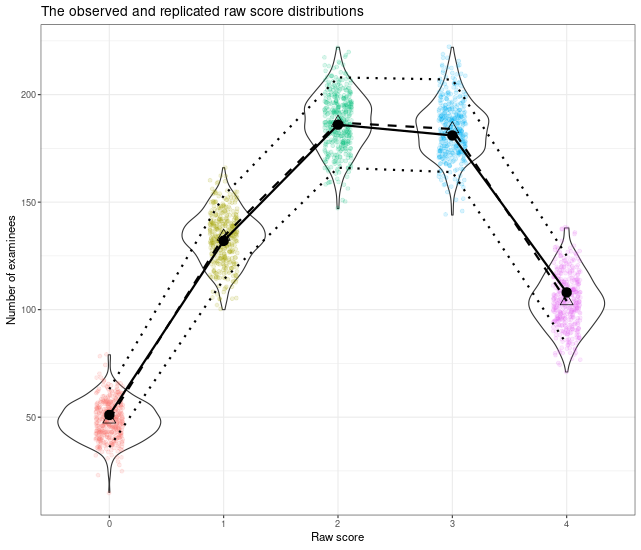
\includegraphics[width=1\columnwidth]{Plots/Plots_2PL_Logit/raw_score_dist.png}
  \caption{Raw Score Distribution for 2PL Logit model. Hollow triangles are posterior predictive medians, while black dots are the number of correct responses to that item.}
  \label{2pl_logit_raw_score}
\end{figure*}

\begin{figure*}[h]
\vspace{-0.5cm}
  \centering
  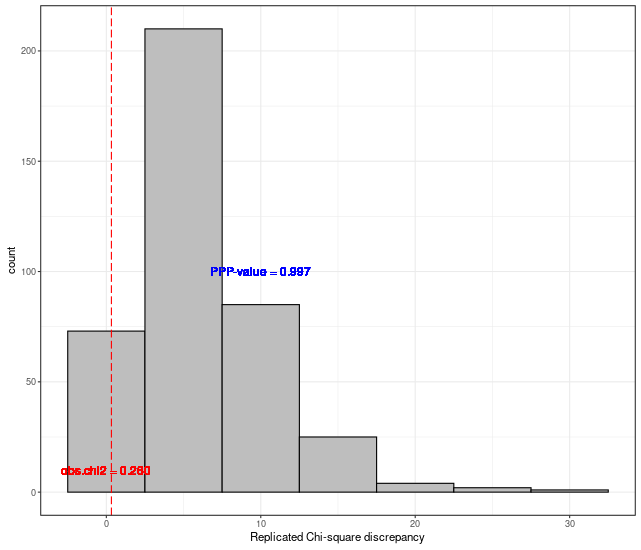
\includegraphics[width=1\columnwidth]{Plots/Plots_2PL_Logit/chi_sqaure.png}
  \caption{Chi Square Discrepancy for 2PL Logit model}
  \label{2pl_logit_chi_squar}
\end{figure*}

\begin{figure*}[h]
\vspace{-0.5cm}
  \centering
  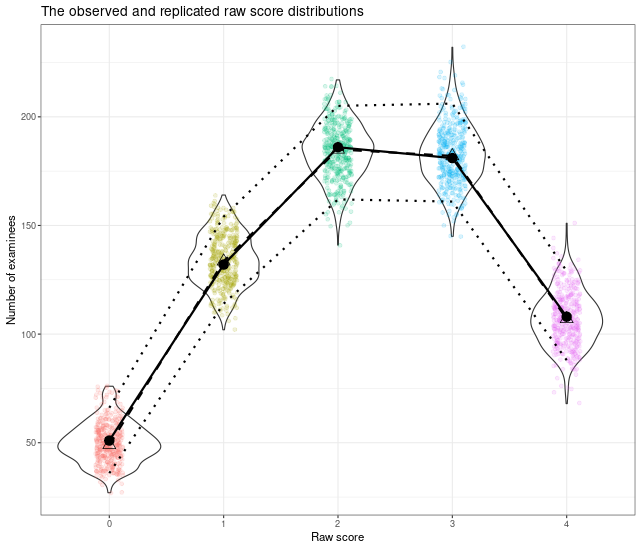
\includegraphics[width=1\columnwidth]{Plots/Plots_2PL_Ogive/raw_score_dist.png}
  \caption{Raw Score Distribution for 2PL Normal Ogive model. Hollow triangles are posterior predictive medians, while black dots are the number of correct responses to that item.}
  \label{2pl_ogive_raw_score}
\end{figure*}

\begin{figure*}[h]
\vspace{-0.5cm}
  \centering
  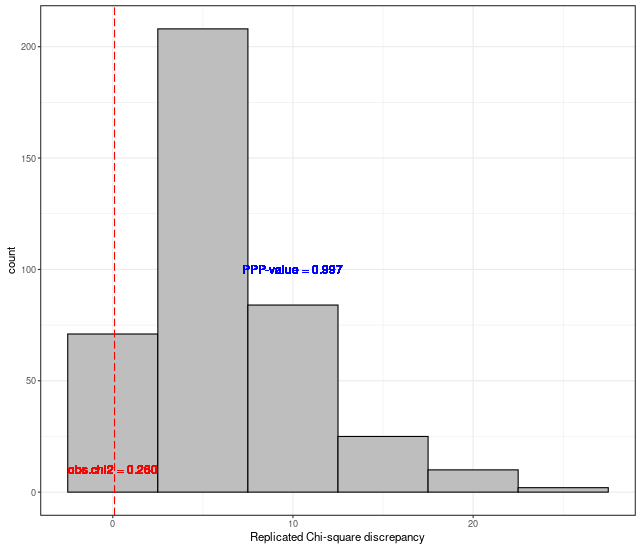
\includegraphics[width=1\columnwidth]{Plots/Plots_2PL_Ogive/chi_square.png}
  \caption{Chi Square Discrepancy for 2PL Normal Ogive model}
  \label{2pl_ogive_chi_squar}
\end{figure*}

\begin{figure*}[h]
\vspace{-0.5cm}
  \centering
  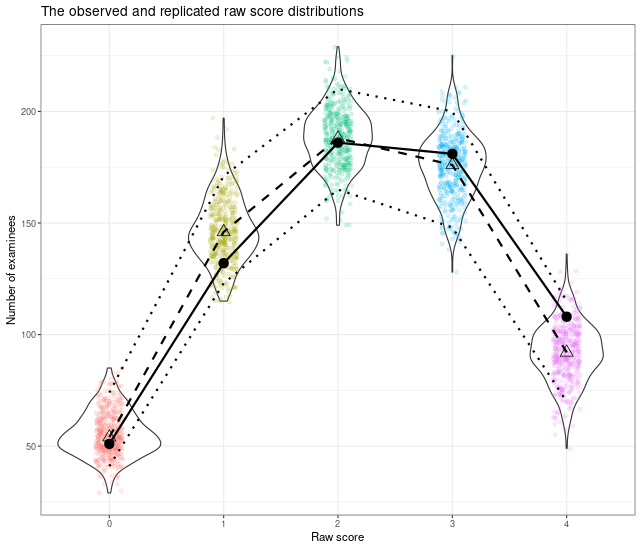
\includegraphics[width=1\columnwidth]{Plots/Plots_2PL_mlirt_Logit/raw_score_dist.png}
  \caption{Raw Score Distribution for 2PL Multilevel Logit model. Hollow triangles are posterior predictive medians, while black dots are the number of correct responses to that item.}
  \label{2pl_logit_mlirt_raw_score}
\end{figure*}

\begin{figure*}[h]
\vspace{-0.5cm}
  \centering
  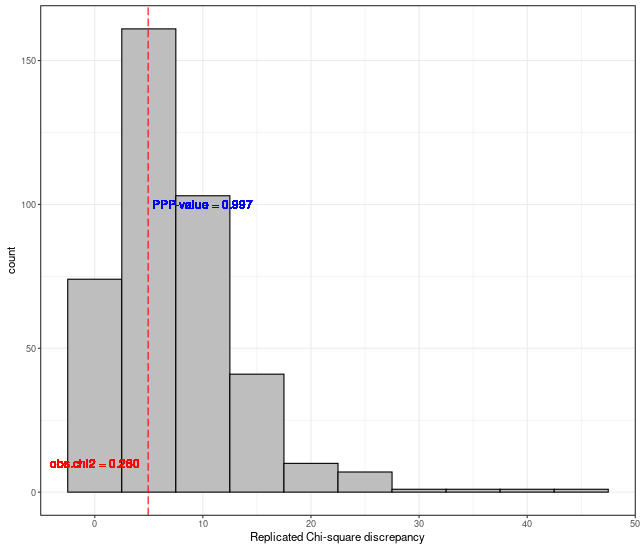
\includegraphics[width=1\columnwidth]{Plots/Plots_2PL_mlirt_Logit/chi_square.png}
  \caption{Chi Square Discrepancy for 2PL Multilevel Logit model}
  \label{2pl_logit_mlirt_chi_squar}
\end{figure*}

\begin{figure*}[h]
\vspace{-0.5cm}
  \centering
  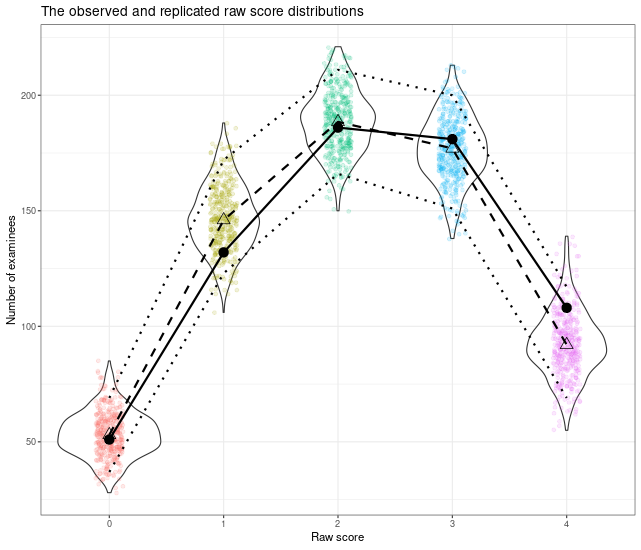
\includegraphics[width=1\columnwidth]{Plots/Plots_2PL_mlirt_Ogive_NC/raw_score_dist.png}
  \caption{Raw Score Distribution for 2PL Multilevel Normal Ogive model. Hollow triangles are posterior predictive medians, while black dots are the number of correct responses to that item.}
  \label{2pl_ogive_nc_mlirt_raw_score}
\end{figure*}

\begin{figure*}[h]
\vspace{-0.5cm}
  \centering
  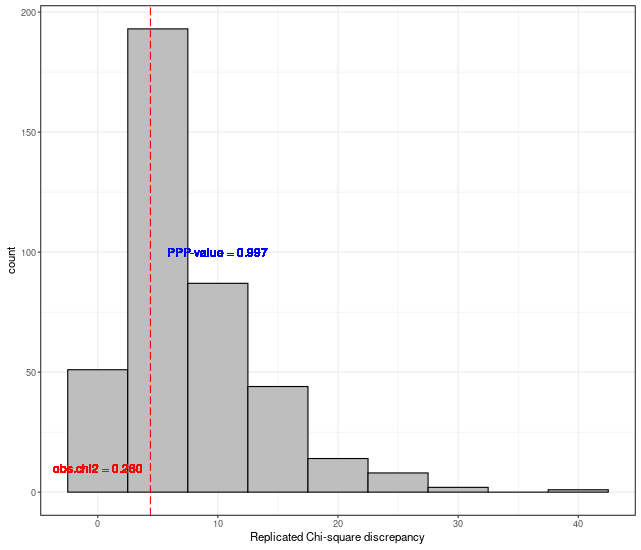
\includegraphics[width=1\columnwidth]{Plots/Plots_2PL_mlirt_Ogive_NC/chi_square.png}
  \caption{Chi Square Discrepancy for 2PL Multilevel Normal Ogive model}
  \label{2pl_ogive_nc_mlirt_chi_squar}
\end{figure*}

\end{document}


